\documentclass[oneside]{book}
\usepackage[T1]{fontenc}
\usepackage[utf8]{inputenc}
\usepackage{geometry}   
\usepackage{float}
\usepackage[section]{placeins}
\usepackage{amsmath}
\usepackage{amssymb}
\usepackage{amsfonts}
\usepackage[colorlinks=true, allcolors=blue]{hyperref}
\usepackage{mathtools}
\usepackage[switch, mathlines]{lineno}
\usepackage[usenames,dvipsnames]{xcolor} 
\usepackage[normalem]{ulem}
\usepackage[capitalise,nameinlink]{cleveref}
\usepackage{enumitem}
\usepackage{csquotes}
\usepackage{xspace}
\usepackage{multirow}
\usepackage{tabularx}
\usepackage{color, colortbl}
\usepackage[colorinlistoftodos]{todonotes}
\usepackage{graphicx}

% for writing code blocks 
\usepackage{listings}
%\usepackage{color}

\definecolor{orange}{rgb}{1,0.5,0}
\definecolor{darkorange}{rgb}{0.69,0.33,0.13}
\definecolor{fidcol}{rgb}{0.7,0,0}
\definecolor{mkcol}{rgb}{0.5,0,0.5}
\definecolor{mmcol}{rgb}{0.7,0.17,0.31}
\definecolor{dscol}{rgb}{0.6,0.1,0.2}
\definecolor{mccol}{rgb}{0.2,0.4,0.6}
\definecolor{darkgreen}{rgb}{0.05,0.5,0.06}
\definecolor{carnelian}{rgb}{0.7, 0.11, 0.11}
\definecolor{dkgreen}{rgb}{0,0.6,0}
\definecolor{mauve}{rgb}{0.58,0,0.82}
%table colors
\definecolor{gray}{gray}{0.9}
\definecolor{cyan}{rgb}{0.88,1,1}

\newcommand*{\Euclid}{\textit{Euclid}\xspace}
\newcommand*{\Planck}{\textit{Planck}\xspace}
\newcommand*{\rd}{\mathrm{d}}
\newcommand*{\rD}{\mathrm{D}}
\newcommand*{\marktodo}{{\color{mmcol} ::TODO::}\xspace}
\newcommand*{\halofit}{\texttt{HALOFIT}\xspace}
\newcommand*{\hmcode}{\texttt{HMCODE}\xspace}
\newcommand*{\montepython}{\texttt MP\xspace}
\newcommand*{\cosmicfish}{\texttt CF\xspace}
\newcommand*{\class}{\texttt CLASS\xspace}
\newcommand*{\camb}{\texttt CAMB\xspace}

\begin{document}
\chapter{Methodology}
The main goal of a forecast is it to figure out how well some experiment will be able to measure some set of parameter. In our case the experiment will be the different probes of the \Euclid mission while the parameter that we want to measure are cosmological parameters. For this we generate some fake data that the experiment could have measured given an underlying fiducial model of the universe, free parameters that show up in our modeling of the data, and of the different survey specifications.\\
The two main methods of forecasting we will deploy in this work are the Markov chain Monte Carlo (MCMC) method and the Fisher Information (FI) method. They are both based in the framework of Bayesian statistics as they are methods of obtaining the posterior distributions, i.e. the probability, $p(\boldsymbol{\theta}|\boldsymbol{D})$, of observing the model parameters, $\boldsymbol{\theta}$, given the data, $\boldsymbol{D}$. The posterior is really what we are after, from it we can extract the mean and the measurement uncertainties of the model parameters. We can group all of our model parameters into 3 groups, cosmological parameters, nuisance parameters, and fixed parameters. While cosmological parameters are really what we are after the nuisance parameters show up during modeling and represent uncertainties in the modeling of the observed data or the observation process itself. In the end they are not of interest to us, so we often only look at the marginal posterior. That is the posterior when the different values of nuisance parameters have been integrated over, i.e \begin{equation}
    \label{eq:bayes-theorem}
    p(\boldsymbol{\theta}_c|\boldsymbol{D}) = \int p(\boldsymbol{\theta}|\boldsymbol{D})\,\rd \boldsymbol{\theta}_n
\end{equation}\\
In this work we will employ Bayesian statistics, where the posterior is related to the likelihood, $\mathcal{L}$, i.e. the probability to measure the data given the parameters. For this we employ the central theorem of Bayesian statistics called the Bayes' theorem. It reads 

\begin{equation}
    p(\boldsymbol{\theta}|\boldsymbol{D}) = \frac{p_\mathrm{rior}(\boldsymbol{\theta})}{E_\mathrm{vidence}(\boldsymbol{D})}\,\mathcal{L}(\boldsymbol{D}|\boldsymbol{\theta}).
\end{equation}
The prior encompasses all of our previous knowledge. It could be either an experimental prior when there was already a measurement of the model parameter done in the past, or it is a theoretical prior. A theoretical prior tell us that the theory requires parameters to be within some bounds, this could be for example the requirement that the neutrino mass is higher than zero or that there are more than zero neutrino species.\\
The Evidence can be understood as the normalization of the likelihood function. It is not accessible with MCMC methods nor FI methods, so we will not go into further details of its  interpretation. We just want to note that it is used when comparing different models to explain the same data. If we obtain the Evidence its value represents the goodness of the fit while also punishing adding additional parameters.\\
In the next sections we will very briefly go over the two different forecasting methods.  
\section{The Markov Chain Monte Carlo Method}
If we wanted to get the posterior from the likelihood we could just use the equation \ref{eq:bayes-theorem}. In reality this is not really feasible as most cosmological problems do not have analytical solutions. Even the most simple problems like comoving distances have no analytical expression once you add dark energy into the mix. This is why we resort to numerical methods like the MCMC method. In this method the goal is to obtain a sequence of random variables lets call them $\{\boldsymbol{\theta}_i|i=1,...,N\}$. In our case these variables will be a vector of our model parameters, but the idea is much more general. When this sequence or chain is marcovian it can be shown that the distributions of the random variables converge to the distributions of the parameters, i.e. the posterior. The requirement marcovian means that each individual element of the chain has a probability that is only a function of the last element of the chain.\\
There are different algorithms to generate such a chain but the most simple one and the one that we use in this work is the Metropolis-Hastings algorithms. The Metropolis-Hastings algorithms starts with a random point in parameter space that is our first chain element $\boldsymbol{\theta}_1$. It then proposes a new point $\boldsymbol{\theta}'$. For the proposal of the new point we typically use some multivariate Gaussian that was our initial guess of the distributions of the parameters $\boldsymbol{\theta}$. We denote the distribution that we sample the point from as $q(\boldsymbol{\theta}'|\boldsymbol{\theta}_1)$.\\
This new point is then accepted with an acceptance probability \begin{equation}
    \label{eq:acceptance-rate}
    A(\boldsymbol{\theta}_1 \to \boldsymbol{\theta}') = \min\left(1,\frac{\mathcal{L}(\boldsymbol{D}|\boldsymbol{\theta}')}{\mathcal{L}(\boldsymbol{D}|\boldsymbol{\theta}_1)}\,\frac{q(\boldsymbol{\theta}_1|\boldsymbol{\theta}')}{q(\boldsymbol{\theta}'|\boldsymbol{\theta}_1)}\right).
\end{equation}
The next element of the chain becomes then either $\boldsymbol{\theta}'$ or stays $\boldsymbol{\theta}_1$ with a probability given by the acceptance probability. This procedure is then iterated until the element of the chain have converged to follow a static distribution.\\
 When the distribution of points, $\pi(\boldsymbol{\theta})$, has become static, the probabilities of going from one point to another need to fulfill the condition of reversibility. This means that the points fulfill \begin{equation}
    \pi(\boldsymbol{\theta}')\, P(\boldsymbol{\theta}'\to\boldsymbol{\theta})= \pi(\boldsymbol{\theta})\,P(\boldsymbol{\theta}\to\boldsymbol{\theta}'),
 \end{equation}
 where $P$ denotes the transition probability to go from one point to the other. This condition is called detailed balance and is an expression of the condition that equilibrium states should not change under time reversal. \\
 If we use our acceptance probability and the suggestion probability to calculate the transition probability we find \begin{equation}
    \pi(\boldsymbol{\theta}')\,q(\boldsymbol{\theta}|\boldsymbol{\theta}')\,A(\boldsymbol{\theta}'\to\boldsymbol{\theta}) = \pi(\boldsymbol{\theta})\,q(\boldsymbol{\theta}'|\boldsymbol{\theta})\,A(\boldsymbol{\theta}\to\boldsymbol{\theta}').
 \end{equation}
 Next we realize that either $A(\boldsymbol{\theta}'\to\boldsymbol{\theta})=1$ or $A(\boldsymbol{\theta}\to\boldsymbol{\theta}')=1$  as the fraction on the right side 
 of equation \ref{eq:acceptance-rate} is reciprocal under the exchange of the states. Without loss of generality we chose that \\$A(\boldsymbol{\theta}'\to\boldsymbol{\theta})=1$ this leads to 
 \begin{align}
    \pi(\boldsymbol{\theta}')\,q(\boldsymbol{\theta}|\boldsymbol{\theta}') &= \pi(\boldsymbol{\theta})\,q(\boldsymbol{\theta}'|\boldsymbol{\theta})\,\frac{\mathcal{L}(\boldsymbol{D}|\boldsymbol{\theta}')}{\mathcal{L}(\boldsymbol{D}|\boldsymbol{\theta})}\,\frac{q(\boldsymbol{\theta}|\boldsymbol{\theta}')}{q(\boldsymbol{\theta}'|\boldsymbol{\theta})} \nonumber \\
    \frac{\pi(\boldsymbol{\theta}')}{\mathcal{L}(\boldsymbol{D}|\boldsymbol{\theta}')} &= \frac{\pi(\boldsymbol{\theta})}{\mathcal{L}(\boldsymbol{D}|\boldsymbol{\theta})}.
 \end{align}
 This means that the static distribution that the points tend converge to is the likelihood up to some constant factor. Inserting this then into equation \ref{eq:bayes-theorem} gives us our posterior up to some factor. This is precisely why when doing the Metropolis-Hastings algorithm there is no way of obtaining the evidence.\\
There is some detail that needs to be said about good convergence of marcovian chains. Firstly to define what we mean with a converged chain there are some metrics that are beeing used in our case we use the Gelman-Rubin test. In this test we launch multiple chains from different starting points, and they all converge to the final distribution of the likelihood. Then we calculate two quantiles. First quantity is the variance of the mean of the chains, i.e. how far apart are the different chains centers from another. The second quantity is the mean of the variance of each chain, i.e. how much are the chains themselves varying from their center. For a converged chain we would expect that the ratio of these two quantities are close to one, so we use this ratio to measure chain convergence.\\
Often denoted as the R-1 test we often require a chain to fulfill 
\begin{equation}
 \mathrm{R}-1 \coloneqq \sqrt{\frac{\mathrm{Var(chain\,means)}}{\mathrm{mean(chain\,variances)}}} -1 \overset{!}{<} 0.1
\end{equation}
to be considered converged. This requires our distribution $q$ from witch we propose points should be already quite close to target distribution $\mathcal{L}$. The reasoning is following, if the suggested points would be way off of the bulk of the likelihood then they would never be accepted and the chain could not move very much. In the ends the individual chains would have very low variances. The opposite effect happens when the proposal distribution would only propose points in the very center of the likelihood, then the chains would accept every suggested. This would make it that firstly the variance of the chain means would be quite high as the random walk would not converge to the center of the likelihood. Secondly this would also have the effect that there could be regions of the likelihood that would never be explored by the chains.\\
To help with the convergence during each run when the chains had enough time to burn in and reached some milestones of convergence we update the proposal distribution. For this we calculate the covariance of the chains and use a multivariate Gaussian with the sample covariance to propose points out of. This has the effect that the main requirement of a marcovian chain gets broken, this is because now the probability to go from one point to the next depends not only on the last point but also on previous points. This means that if we want to analyze the chains we need to always throw away the points of the chains before the last update of the proposal distribution.\\
The code that we use to run our MCMC is called MontePython ({\tt MP}) and has two modes that are of interest to us. The first mode is the Metropolis-Hastings mode, it uses the same strategy that was discussed earlier to generate the chains where we also update the proposal distribution to have fast convergence. The second mode is the Fisher mode that is discussed in the next section. The reason why we use both modes of \montepython will become clearer in the Chapter about Validation.  
\section{The Fisher Information Method}
We observe that for well constrained parameters the posterior looks often times like a multivariate Gaussian. The FI method employs this in that it is an approximation where the Gaussian is tailored onto the likelihood and then the error is extracted from the Gaussian. The Idea of the formalism is the following: To parametrize a multivariate Gaussian you only need the covariance matrix, $C$, and the mean of the variables, $\boldsymbol{\mu}$. In our case the variables would be cosmological parameter and the covariance then would contain the measurement uncertainties.\\
Assuming that the posterior can be approximated as a Gaussian we can write it as \begin{equation}
    p(\boldsymbol{\theta}|\boldsymbol{D}) \propto p_\mathrm{rior}(\boldsymbol{\theta})\,\mathcal{L}(\boldsymbol{D}|\boldsymbol{\theta}')\approx \mathcal{N}\,\exp\left[-\frac{1}{2}\,\left(\boldsymbol{\theta}-\boldsymbol{\mu}\right)\cdot C^{-1}\,\left(\boldsymbol{\theta}-\boldsymbol{\mu}\right)\right].
\end{equation}
For a Gaussian posterior the mean is also at the best fit, this is why when we do a forecast we directly know the value of $\boldsymbol{\mu}$. It is the value of the model parameters at the fiducial point where we generated our fake data. We can now use that the covariance can be extract from the log of the posterior by calculating the second derivative. It is \begin{equation}
    \left.-\frac{\partial^2}{\partial \theta_i\,\partial \theta_j}\log(p(\boldsymbol{\theta}|\boldsymbol{D}))\right|_{\boldsymbol{\theta}=\boldsymbol{\mu}}\approx\left(C^{-1}\right)_{ij}. 
\end{equation}
If we assume flat priors in the region of interest we can directly calculate the derivative of the likelihood. This leads to the definition of the Fisher Information matrix as \begin{equation}
    F_{ij}\coloneqq -\frac{\partial^2}{\partial \theta_i\,\partial \theta_j}\log\mathcal{L}(\boldsymbol{D}|\boldsymbol{\theta})
\end{equation}
For Gaussian priors we can just add the term later. We will discuss later on how to do that when we discuss adding different experiments. Non-Gaussian or flat priors are harder to approximate. The easiest method of dealing with exponential priors is to make it a flat prior by transforming the relevant parameters into log space. This might make the contours less Gaussian depending on how well constrained the parameter are.\\
The difficulty of FI method is that often times it is not so clear how to obtain the second order derivatives of the likelihood. There are some codes that were purposefully build to be differentiable i.e. that you can obtain the derivates for free. The typical Einstein-Boltzmann solvers (EBS) {\tt ClASS} and {\tt CAMB} do not have that functionality, so we need to obtain the derivatives numerically. This is what \montepython does in Fisher mode. We calculate the second order derivates using a double sided finite differences scheme. We note numerical derivatives with the symbol D, thus we can write 
\begin{align}
    \frac{\rD^2 \log\mathcal{L}}{\rD \theta_i \, \rD \theta_j} =& \frac{1}{4\,h_i\,h_j}\left[\log\mathcal{L}(\theta_i+h_i,\theta_j+h_j)-\log\mathcal{L}(\theta_i+h_i,\theta_j-h_j)\right. \nonumber\\
&-\left.\log\mathcal{L}(\theta_i-h_i,\theta_j+h_j)+\log\mathcal{L}(\theta_i-h_i,\theta_j-h_j)\right]\quad \text{for}\,i\neq j\\
    \frac{\rD^2 \log\mathcal{L}}{\rD^2 \theta_i} =&  \frac{1}{h_i^2} \left[\log\mathcal{L}(\theta_i+h_i)+\log\mathcal{L}(\theta_i-h_i)-2\,\log\mathcal{L}(\theta_i)\right],
\end{align}
where we have left out the arguments of the log likelihood that do not get varied in each line. Here the advantage of using the FI method becomes clear, while the MCMC often times needs multiple thousand calls of the EBS the FI method needs much less. In the Implementation we use for $N$ parameters we have to call the likelihood $2\,N$ times for the diagonal elements and $2\,N\,(N-1)$ times for the off diagonal elements, making our total calls $2\,N^2$. Even then we can shave off some more time if we use that when varying nuisance parameters there is no need for calling the EBS anymore.\\
The calculation of the second derivative is numerically quite sensitive to the choice of stepsize. It was shown before in \marktodo that the optimal stepsize to calculate the derivatives is of the order of few percents of the marginalized error. And even then one needs to use very high precision settings of the EBS to be able to have stable results. This does defeat the purpose of the FI method as to obtain the marginalized error we would need to run an MCMC.\\
To make the computation of the FI matrix numerically stable we can use the explicit form of the photometric and spectroscopic likelihoods to write it using only first derivates of the observables. For the photometric likelihood we find \begin{equation}
    F_{ij} = \frac{1}{2}\,\sum_{\ell=\ell_\mathrm{min}}^{\ell_\mathrm{max}} (2\,\ell+1)\,f_\mathrm{sky}\,\mathrm{Tr}\left[\left(C_\ell^\mathrm{fid}\right)^{-1}\,\left(\left.\partial_i C^\mathrm{th}_\ell\right|_\mathrm{fid}\right)\,\left(C_\ell^\mathrm{fid}\right)^{-1}\,\left(\left.\partial_j C^\mathrm{th}_\ell\right|_\mathrm{fid}\right)\right].
\end{equation}
We have replaced the observed angular power spectrum with the theoretical angular power spectrum calculated at the fiducial like in the spectroscopic probe. There are two advantages of calculating the FI matrix like this, firstly the derivatives that show up are first order and thus much easier to calculate. To calculate them we use either of two finite differences stencils 
\begin{align}
\frac{\rD C^\mathrm{th}_\ell}{\rD \theta_i} &= \frac{1}{2\,h_i}\left[C^\mathrm{th}_\ell(\theta_i+h_i)-C^\mathrm{th}_\ell(\theta_i-h_i)\right]\\
\text{or}\quad&= \frac{1}{6\,h_i}\left[-11\,C^\mathrm{th}_\ell(\theta_i)+18\,C^\mathrm{th}_\ell(\theta_i+h_i)-9\,C^\mathrm{th}_\ell(\theta_i+2\,h_i)+2\,C^\mathrm{th}_\ell(\theta_i+3\,h_i)\right].
\end{align}
By default, we will stick to the double-sided finite difference and not to the one-sided one but to check the numerical stability of our derivatives we have tested both methods. First order derivatives have the property to be more numerically stable. That is why we do not need to tune our stepsize as much as in the case of the second order derivatives. We always use a relative stepsize of 1\% for the cosmological parameters expect for the neutrino mass, where we vary it by a relative 10\%. The choice for the neutrinos stems from the fact, that the neutrino mass only has a small effect on our observables. For a 1\% change of the neutrino mass the change of the observables would be dominated by numerical noise, so we had to choose a higher stepsize. We will also test that the choice of a 10\% stepsize for massive neutrinos produces stable result.\\
The second advantage of this method is that to compute all derivatives one only needs to call the code $2\,N$ since the first order derivates of the observables can then be multiplied to find the second order derivates of the likelihood.\\
For the spectroscopic likelihood we find a similar expression for the likelihood \begin{equation}
    F_{ij} = \frac{1}{8\,\pi^2}\sum_i \int k_\mathrm{fid}^2 \,\partial_i \left[\log P_\mathrm{th}(k_\mathrm{fid},\mu_\mathrm{fid},z_i) \right|_\mathrm{fid}\,\,\partial_i \left[\log P_\mathrm{th}(k_\mathrm{fid},\mu_\mathrm{fid},z_i)\right|_\mathrm{fid}\,V_i^\mathrm{fid} \rd k_\mathrm{fid} \rd \mu_\mathrm{fid}  .
\end{equation}
Again we find that the FI matrix can be written with products of fist order derivatives. To calculate the FI matrix for our forecast we will use the code Cosmicfish ({\tt CF}) that we have modified such that our changes to the recipes of the observables are consistent with our \montepython Implementation. Since \cosmicfish never calculates the actual likelihood this gives us a great test for our likelihood Implementation, if the FI matrix obtained by \montepython in Fisher mode agrees with the FI matrix from \cosmicfish. This is further discussed in the chapter \marktodo about the Validation.\\
Finally, the FI formalism gives us a guiding principle to make educated guesses for the proposal distributions. Firstly when we have already a covariance matrix of a previous MCMC, and we want to launch another MCMC but with fewer parameters, then just deleting the files corresponding rows is not optimal but was the Implementation in \montepython. We have added a new method of fixing that leads to a better initial guess.\\
We calculate a matrix from the covariance of the MCMC that is approximating the FI matrix by just inverting it. The matrix now has all parameters that the actual Fisher would have. Now the if we remind ourselves of the definition of the FI matrix as the second derivate of the log likelihood then fixing a parameter is the same as never adding the corresponding lines to the matrix. Inversion then leads us to the desired covariance matrix. We illustrate this procedure below.
\begin{equation}
    \bordermatrix{~ & \boldsymbol{\theta}_o && \boldsymbol{\theta}_f \cr
    \boldsymbol{\theta}_o &C_{oo}&& C_{of}\cr
    \cr
    \boldsymbol{\theta}_f &C_{fo}&& C_{ff}\cr } \overset{\mathrm{invert}}{\longrightarrow}     
    \bordermatrix{~ & \boldsymbol{\theta}_o && \boldsymbol{\theta}_f \cr
    \boldsymbol{\theta}_o &F_{oo}&& F_{of}\cr
    \cr
    \boldsymbol{\theta}_f &F_{fo}&& F_{ff}\cr } {\overset{\mathrm{extract}}{\longrightarrow}} F_{oo} \overset{\mathrm{invert}}{\longrightarrow} \tilde{C}_{oo} \nonumber
\end{equation}
We have denoted the parameters we want to keep open with $\boldsymbol{\theta}_o$ and the parameters we want to fix with $\boldsymbol{\theta}_f$. In the Fisher approximation the new covariance $\tilde{C}_{oo}$ is the covariance of the MCMC if the parameters had been fixed from the beginning. This also gives us an interpretation of what the diagonal elements of the Fisher mean. If we were to fix all parameters expect of one then the matrix $F_{oo}$ is just a number. The inversion is then just its reciprocal value but the interpretation of this number would be the variance when every other parameter was fixed. This is precisely what the unmarginalized error is thus the diagonal of a Fisher contains the reciprocal unmarginalized errors.\\
Next we can ask ourselves the question on how to add multiple experiments together. On the level of the likelihood when neglecting cross correlation the likelihood of a combined probe, $\mathcal{L}$, factorizes into the likelihoods of the individual probes,$\mathcal{L}^1$ and $\mathcal{L}^2$. For the Fisher we thus can write 
\begin{equation}
    F_{ij} = \frac{\partial^2}{\partial \theta_i\,\partial \theta_j} \log \mathcal{L} = \frac{\partial^2}{\partial \theta_i\,\partial \theta_j} \left[\log \mathcal{L}^1 + \log\mathcal{L}^2\right] = F^1_{ij} + F^2_{ij}.
\end{equation}
This means that combining two uncorrelated probes is the same as adding their fisher matrix. We can again use this to get a make an educated guess on the proposal distribution of an MCMC with combined probes, like the spectroscopic and the photometric probes, when there are previous runs. Firstly we have to separate all of our parameters into parameters that are common to both likelihoods $\boldsymbol{\theta}_c$, i.e. the cosmological parameters, and then the nuisance parameters of both likelihoods $\boldsymbol{\theta}_1$ and $\boldsymbol{\theta}_2$. Calculating the derivates of one likelihood with respect to the nuisance parameters of the other likelihood makes little sense but could be done mathematically. The derivatives would just vanish so the Fisher Matrix would have empty rows of zeros in these and would be not invertible. But this helps us in the formulation of our recipe.\\
We start by inverting our MCMC covariance matrices to have the approximate FI matrices. We then add columns and rows of zeros that correspond to the nuisance parameters of the other likelihood. Finally, we can add the matrices and invert the result to get our new guess for the proposal covariance. Typically, this works very well for complimentary probes since breaking degeneracies makes the final posterior Gaussian enough for the approximation. We illustrate the final combination recipe below 
\begin{align*}
    \bordermatrix{~ & \boldsymbol{\theta}_c && \boldsymbol{\theta}_1 \cr
    \boldsymbol{\theta}_c &C^1_{cc}&& C^1_{c1}\cr
    \cr
    \boldsymbol{\theta}_1 &C^1_{1d}&& C^1_{11}\cr } \quad ,\quad 
    \bordermatrix{~ & \boldsymbol{\theta}_c && \boldsymbol{\theta}_2 \cr
    \boldsymbol{\theta}_c &C^2_{cc}&& C^2_{c2}\cr
    \cr
    \boldsymbol{\theta}_2 &C^2_{2c}&& C^2_{22}\cr } \overset{\mathrm{invert}}{\longrightarrow}
    \bordermatrix{~ & \boldsymbol{\theta}_c && \boldsymbol{\theta}_1 \cr
    \boldsymbol{\theta}_c &F^1_{cc}&& F^1_{c1}\cr
    \cr
    \boldsymbol{\theta}_1 &F^1_{1d}&& F^1_{11}\cr } \quad ,\quad 
    \bordermatrix{~ & \boldsymbol{\theta}_c && \boldsymbol{\theta}_2 \cr
    \boldsymbol{\theta}_c &F^2_{cc}&& F^2_{c2}\cr
    \cr
    \boldsymbol{\theta}_2 &F^2_{2c}&& F^2_{22}\cr }\\
    \\
    \overset{\mathrm{add\,zeros}}{\hookrightarrow}
    \bordermatrix{~ & \boldsymbol{\theta}_c && \boldsymbol{\theta}_1  &&\boldsymbol{\theta}_2 \cr
    \boldsymbol{\theta}_c &F^1_{cc}&& F^1_{c1} && 0\cr
    \cr
    \boldsymbol{\theta}_1 &F^1_{1d}&& F^1_{11}&& 0\cr 
    \cr
    \boldsymbol{\theta}_2& 0&&0&&0} \quad,\quad 
    \bordermatrix{~ & \boldsymbol{\theta}_c && \boldsymbol{\theta}_1  &&\boldsymbol{\theta}_2 \cr
    \boldsymbol{\theta}_c &F^2_{cc}&&0  && F^2_{c2}\cr
    \cr
    \boldsymbol{\theta}_1 &0&& 0&& 0\cr 
    \cr
    \boldsymbol{\theta}_2& F^2_{2d}&&0&&F^2_{22}} \overset{\mathrm{add}}{\longrightarrow}
    \bordermatrix{~ & \boldsymbol{\theta}_c && \boldsymbol{\theta}_1  &&\boldsymbol{\theta}_2 \cr
    \boldsymbol{\theta}_c &F^1_{cc}+F^2_{cc}&&F^1_{c1}  && F^2_{c2}\cr
    \cr
    \boldsymbol{\theta}_1 &F^1_{1c}&& F^1_{11}&& 0\cr 
    \cr
    \boldsymbol{\theta}_2& F^2_{2d}&&0&&F^2_{22}}\\
    \\
    \overset{\mathrm{invert}}{\hookrightarrow} \tilde{C}
\end{align*}
This also explains how to add a Gaussian prior to a Fisher afterwards when looking at the Bayes theorem \ref{eq:bayes-theorem} again. The prior can be pulled into the likelihood and act like an effective second experiment. The covariance matrix of the multivariate Gaussian prior directly defines a FI matrix that can be just added like an experiment afterwards. This of course needs the prior to be centered on the fiducial cosmology of the forecast.\\
A script to merge covariance matrices for \montepython was added by us. To show how well this works we have combined two test MCMCs of the two main \Euclid probes and present the results in figure . We generated this plot with the use of GetDist \footnote{\href{https://getdist.readthedocs.io}{https://getdist.readthedocs.io}} \marktodo.
\begin{figure}
    \centering
    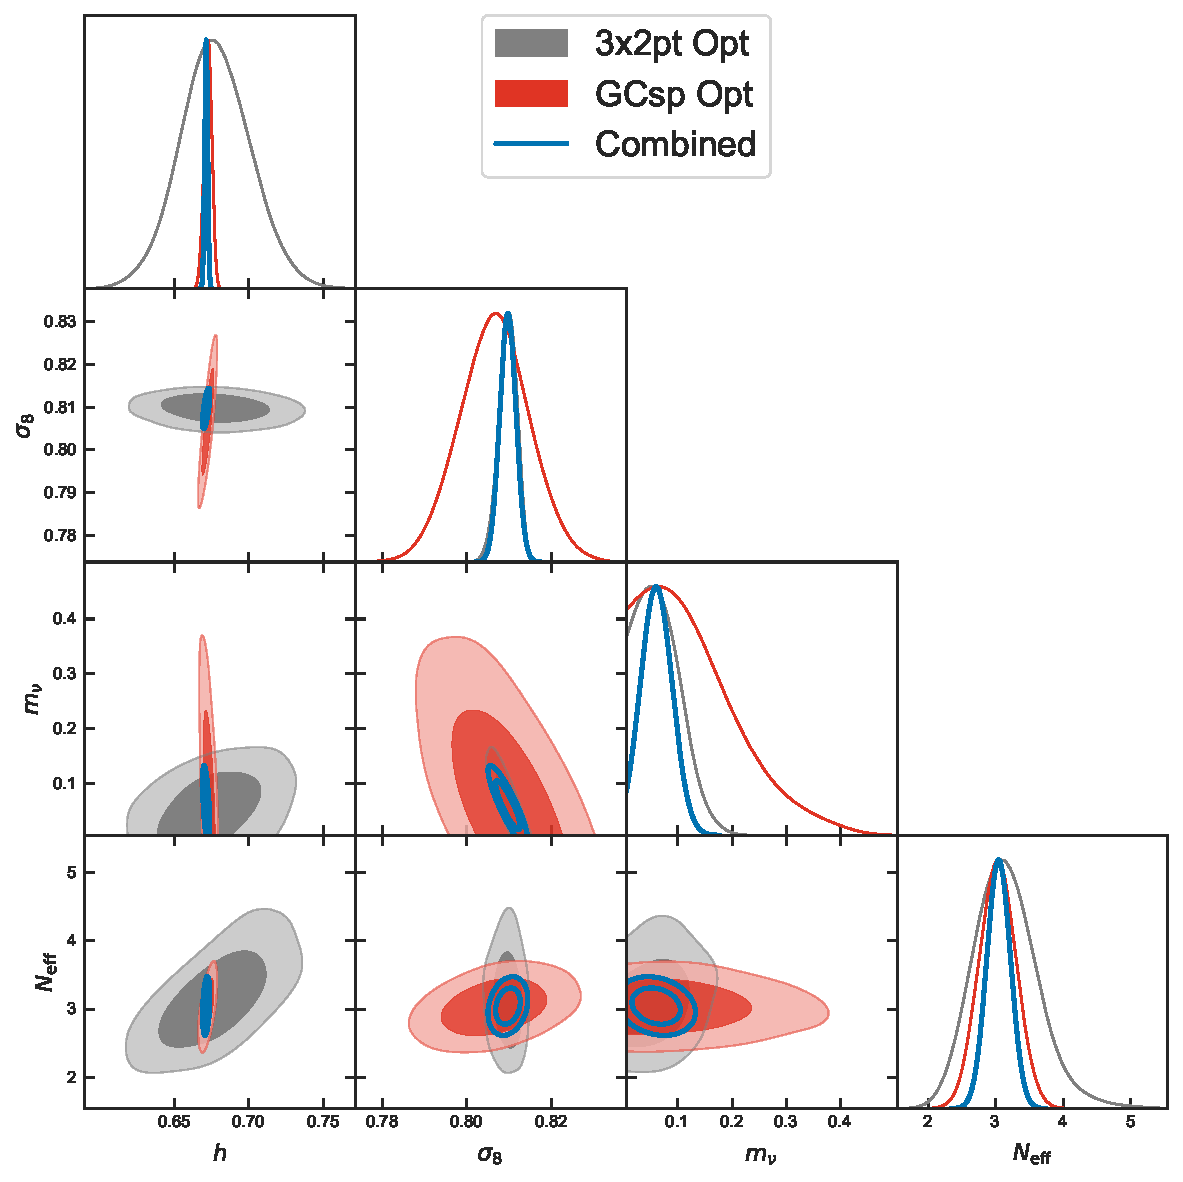
\includegraphics[width=\linewidth]{combined_probes_mnu+Neff_cosmo_test_smoothing.pdf}
    \label{fig:combining-probes}
    \caption{Demonstration of the covariance combination recipe. The MCMCs are done with the settings of the Validation section. The combined probe is not an MCMC, but the ellipses from the Gaussian approximation obtained with the recipe. This also demonstrates very well the complementarity of the \Euclid probes.}
\end{figure}
\end{document}